\documentclass[a4paper,14pt]{extarticle}
\usepackage{mysettings} % Include custom settings

\begin{document}

\thispagestyle{empty} 
% title.tex
\begin{center}
  Министерство образования Республики Беларусь \\
  \bigskip
  Учреждение образования \\
  "<БЕЛОРУССКИЙ ГОСУДАРСТВЕННЫЙ УНИВЕРСИТЕТ ИНФОРМАТИКИ И РАДИОЭЛЕКТРОНИКИ"> \\
  \bigskip \bigskip
  Факультет компьютерных сетей и систем \\
  Кафедра электронных вычислительных средств \\
  \bigskip \bigskip \bigskip \bigskip \bigskip \bigskip \bigskip \bigskip \bigskip \bigskip \bigskip \bigskip
  Отчет по лабораторной работе № 1 \\
  \bf{"<Тема лабораторной работы">}\normalfont \\
  \bigskip \bigskip \bigskip \bigskip \bigskip \bigskip \bigskip \bigskip \bigskip \bigskip \bigskip \bigskip
  \begin{table}[ht]
    \begin{tabular}{p{7cm} p{1cm} p{7cm}}
        Выполнили студенты гр. X5070X \par XXX X.X. \par XXX X.X.\par XXX X.X.& \hfill & \hspace*{30 mm}Проверил \par \hspace*{29 mm} XXX X.X.
    \end{tabular}
  \end{table}
  \vfill \vfill
  \centerline{Минск 2025}
\end{center}
\newpage
  % Include title
\setcounter{page}{2}

\section*{1 ЦЕЛЬ И ЗАДАЧИ ЛАБОРАТОРНОЙ РАБОТЫ}
  1 Изучить влияние параметров дискретизации и разрядности квантования сигналов в
системах мультимедиа.

  2 Разработать MATLAB-модель последовательного АЦП в соответствии с вариантом
задания.

  3 Изучить способы изменения частоты дискретизации (децимация и интерполяция)
аудиосигналов.

  4 Разработать MATLAB-модель, изменяющую частоту дискретизации сигнала в
соответствии с вариантом задания.

\section*{2 РЕЗУЛЬТАТЫ ВЫПОЛНЕНИЯ РАБОТЫ}
\subsection*{2.1 Задание 1}
  Необходимо разработать MATLAB-функцию последовательного АЦП в
соответствии с алгоритмом его работы.

\lstinputlisting[language=TeX]{code/functions/serial_adc.m}

\subsection*{2.2 Задание 2}
При помощи разработанной функции serial\_adc необходимо 
выполнить квантование гармонического сигнала в соответствии с 
вариантом. При помощи функций stem и stairs построить графики 
квантованного сигнала $s_q(n)$ для указанных в варианте
значений $N$ и наложить их на график функции $s(n)$.

\[s(n) = \cos(\dfrac{2\pi20}{12000}n) + \sin(\dfrac{2\pi450}{12000}n - \dfrac{\pi}{8})\]

\lstinputlisting[language=TeX]{code/task2.m}

  Результат выполнения квантования представлен 
на рисунке 1.
\begin{center}
  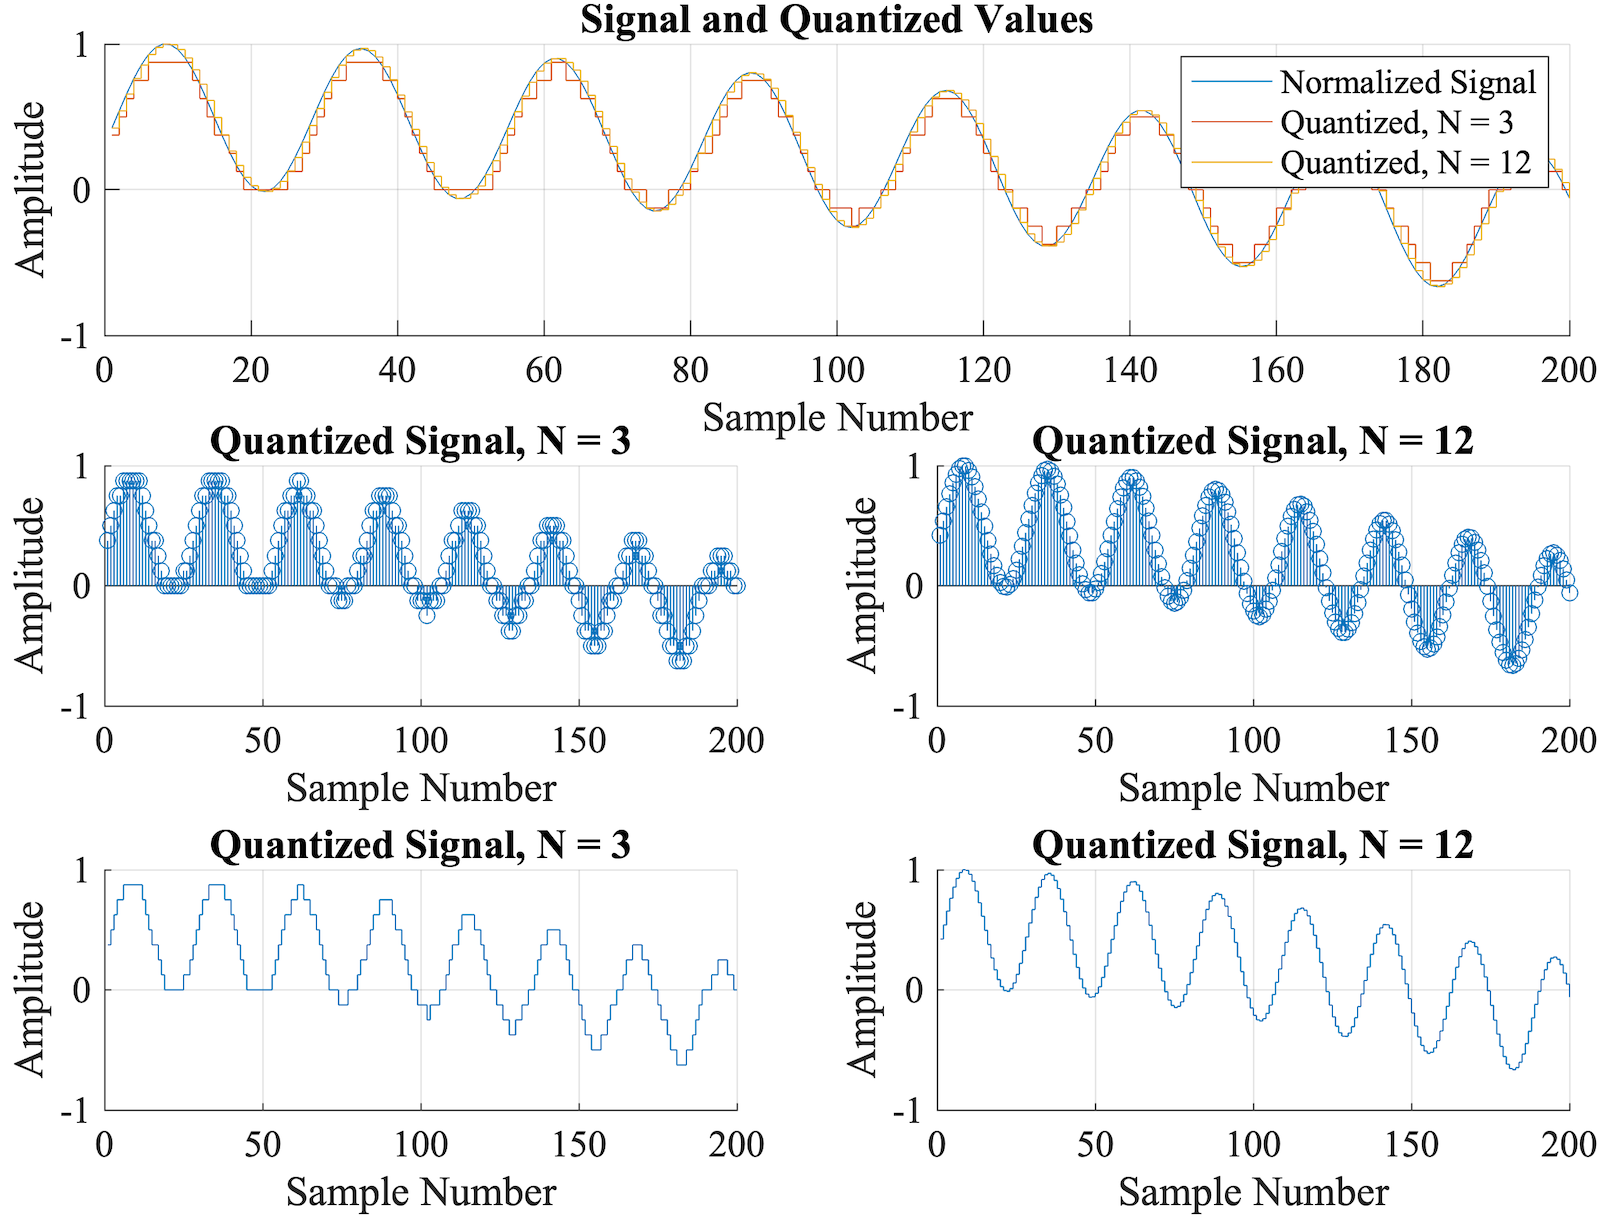
\includegraphics{img/Task_2.png}
  \captionof{figure}{Сигнал при N = 3 и N = 12}
\end{center}

\subsection*{2.3 Задание 3}
Необходимо построить графики ошибки квантования для квантованного сигнала
$s_q(n)$ для указанных в варианте разрядностей $N$. 

\lstinputlisting[language=TeX]{code/task3.m}

  Результат вычисления ошибки представлен 
на рисунке 2.
\begin{center}
  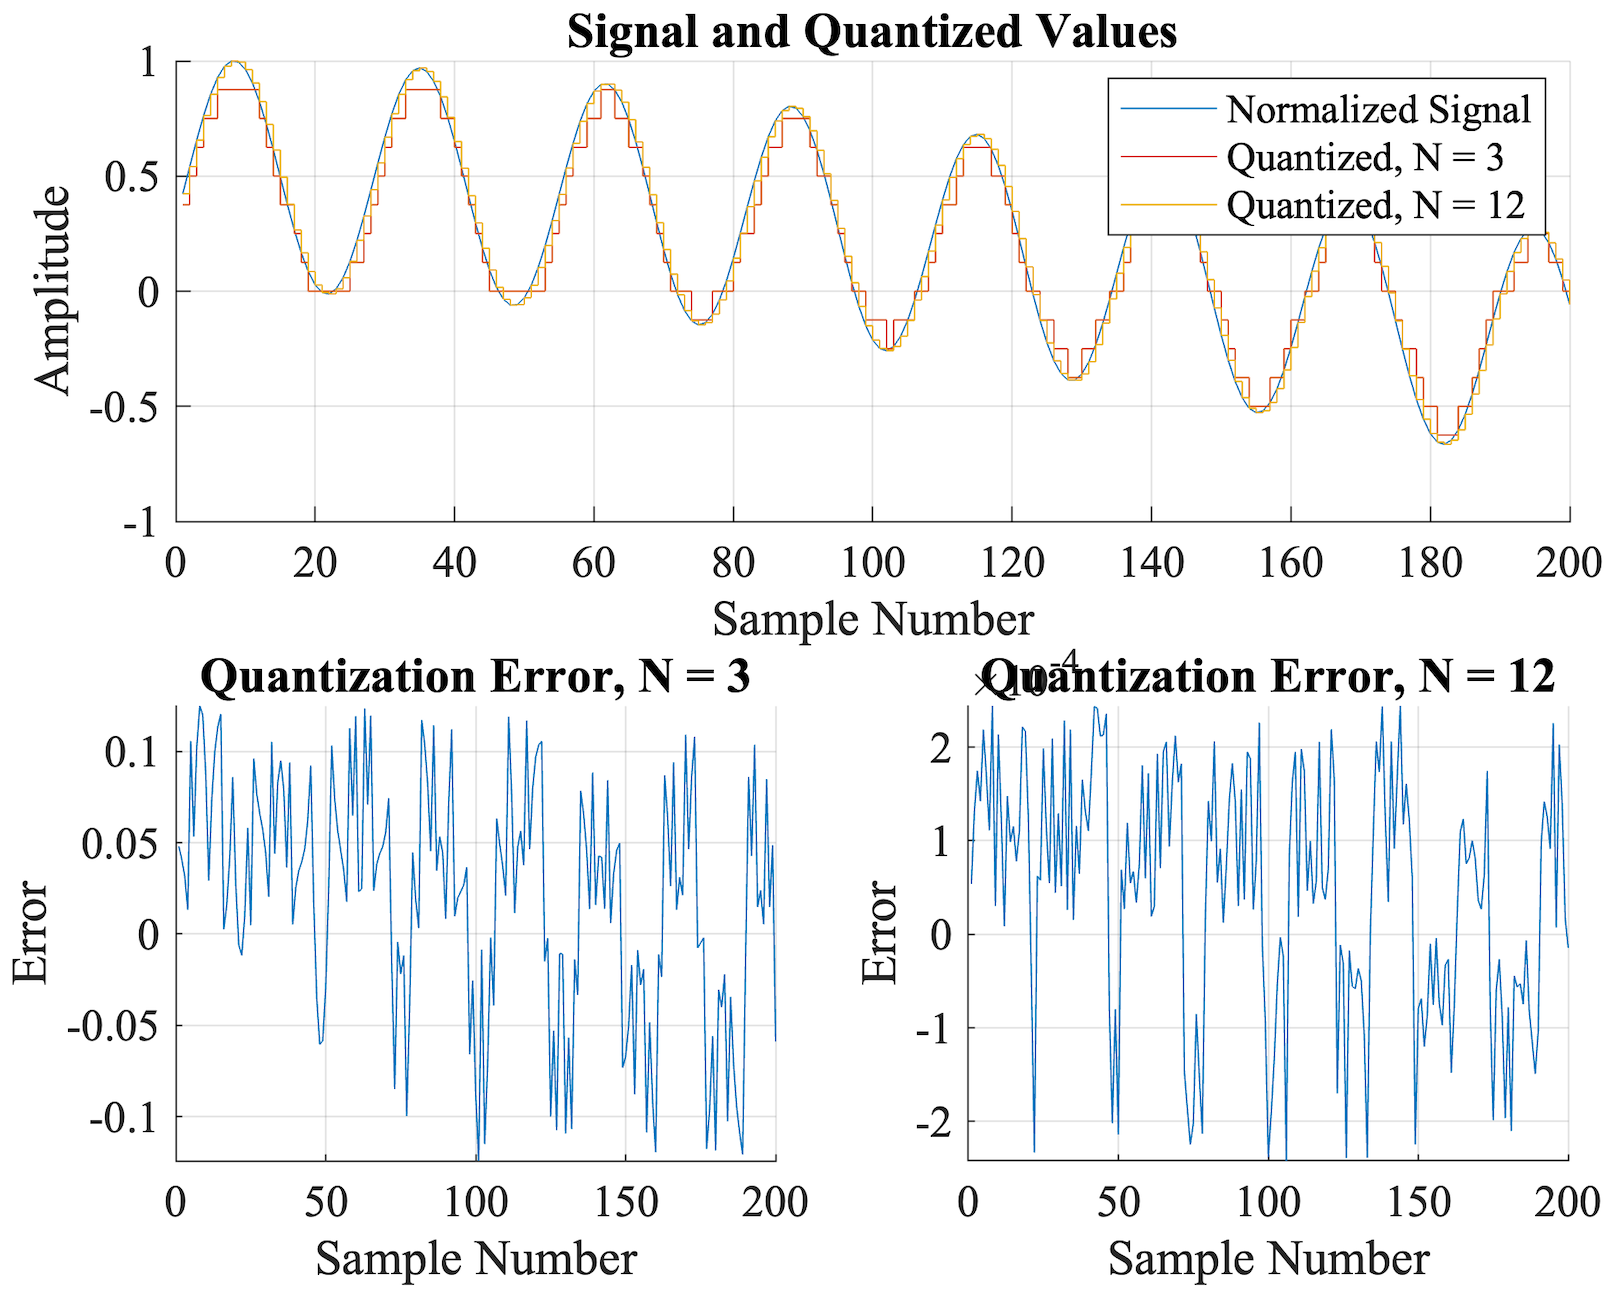
\includegraphics{img/Task_3.png}
  \captionof{figure}{Ошибка квантования для N = 3 и N = 12}
\end{center}

\subsection*{2.4 Задание 4}
Расчёт антиалайзингового фильтра для децимации и интерполяции.
Порядок фильтра $N$ = 100.

\lstinputlisting[language=TeX]{code/task4.m}

  Результат построения фильтра представлен 
на рисунке 3.
\begin{center}
  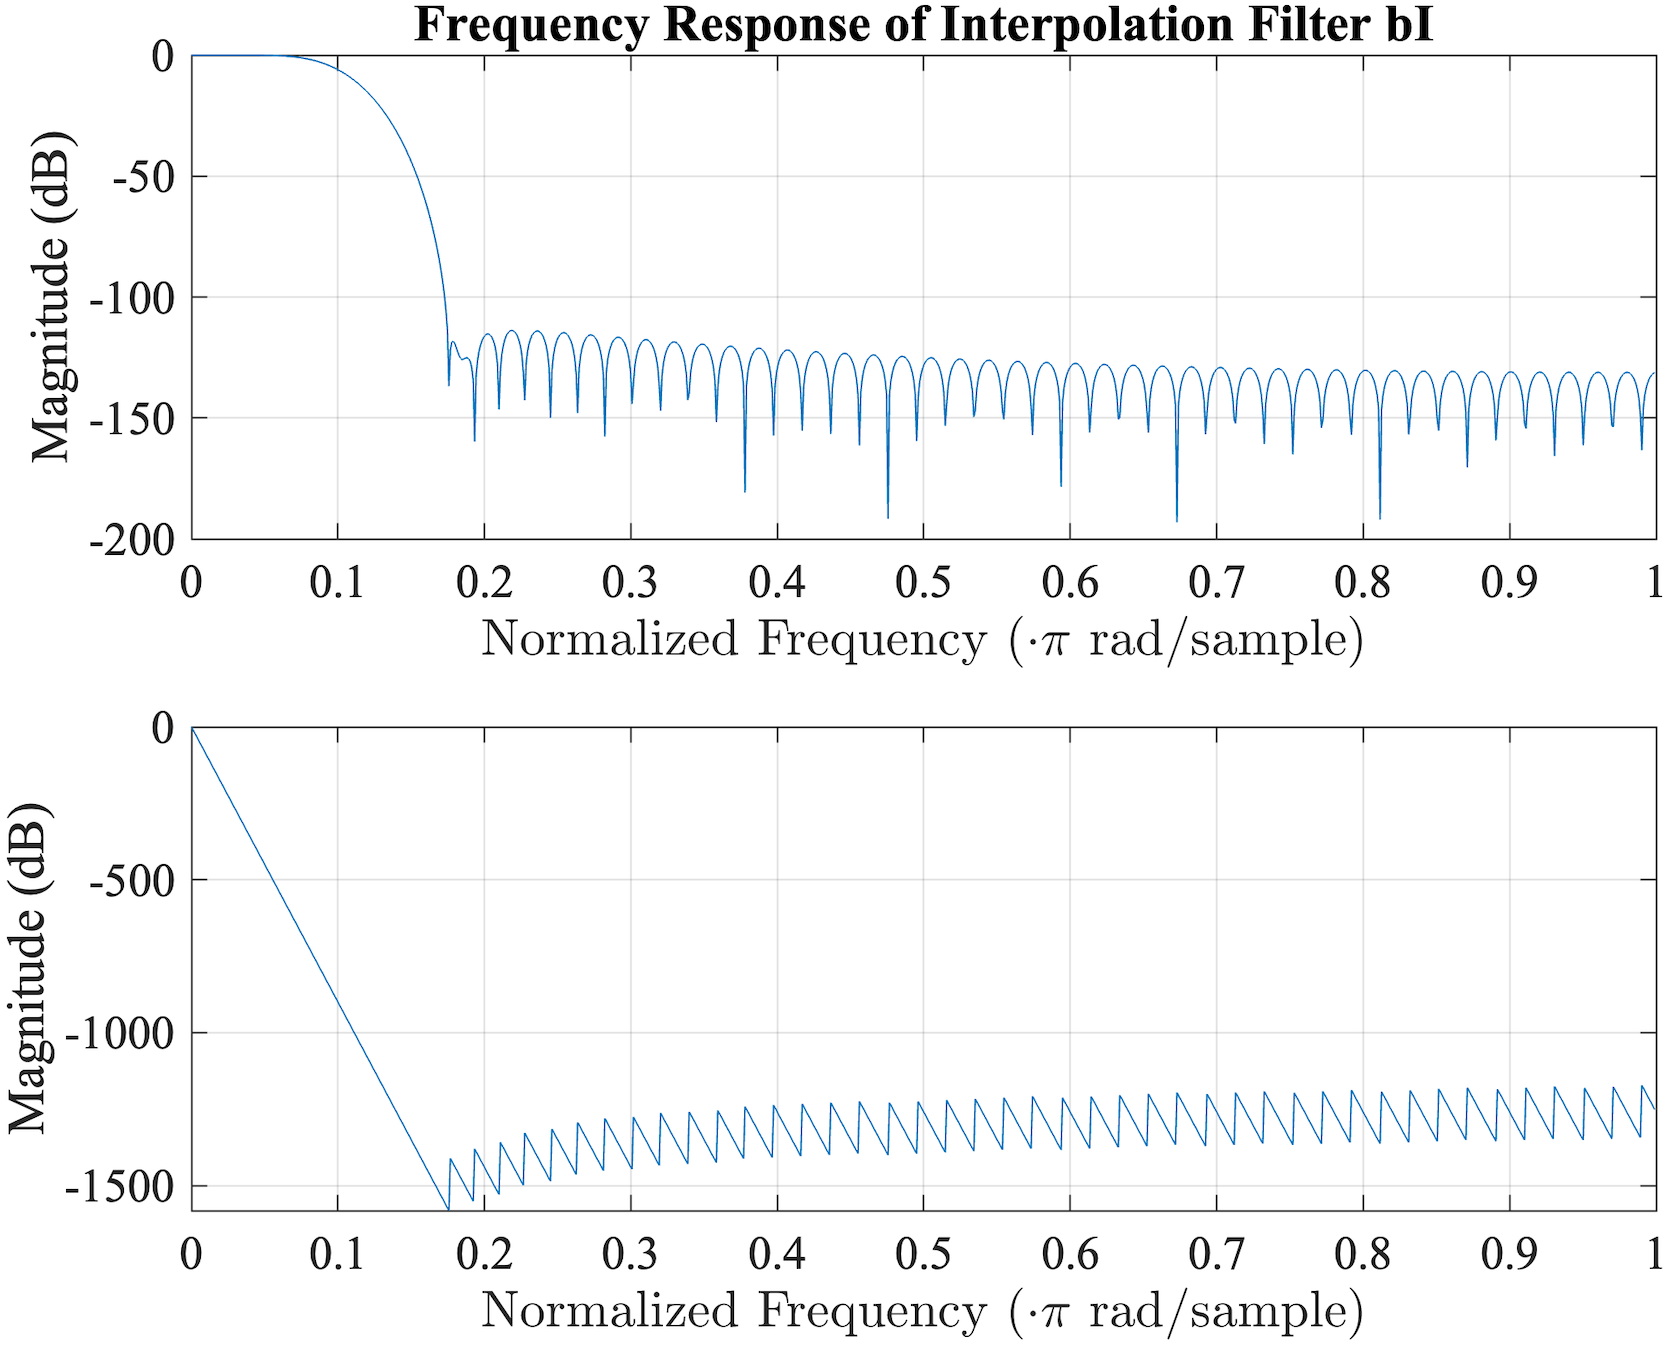
\includegraphics{img/Task_4_1.png}
  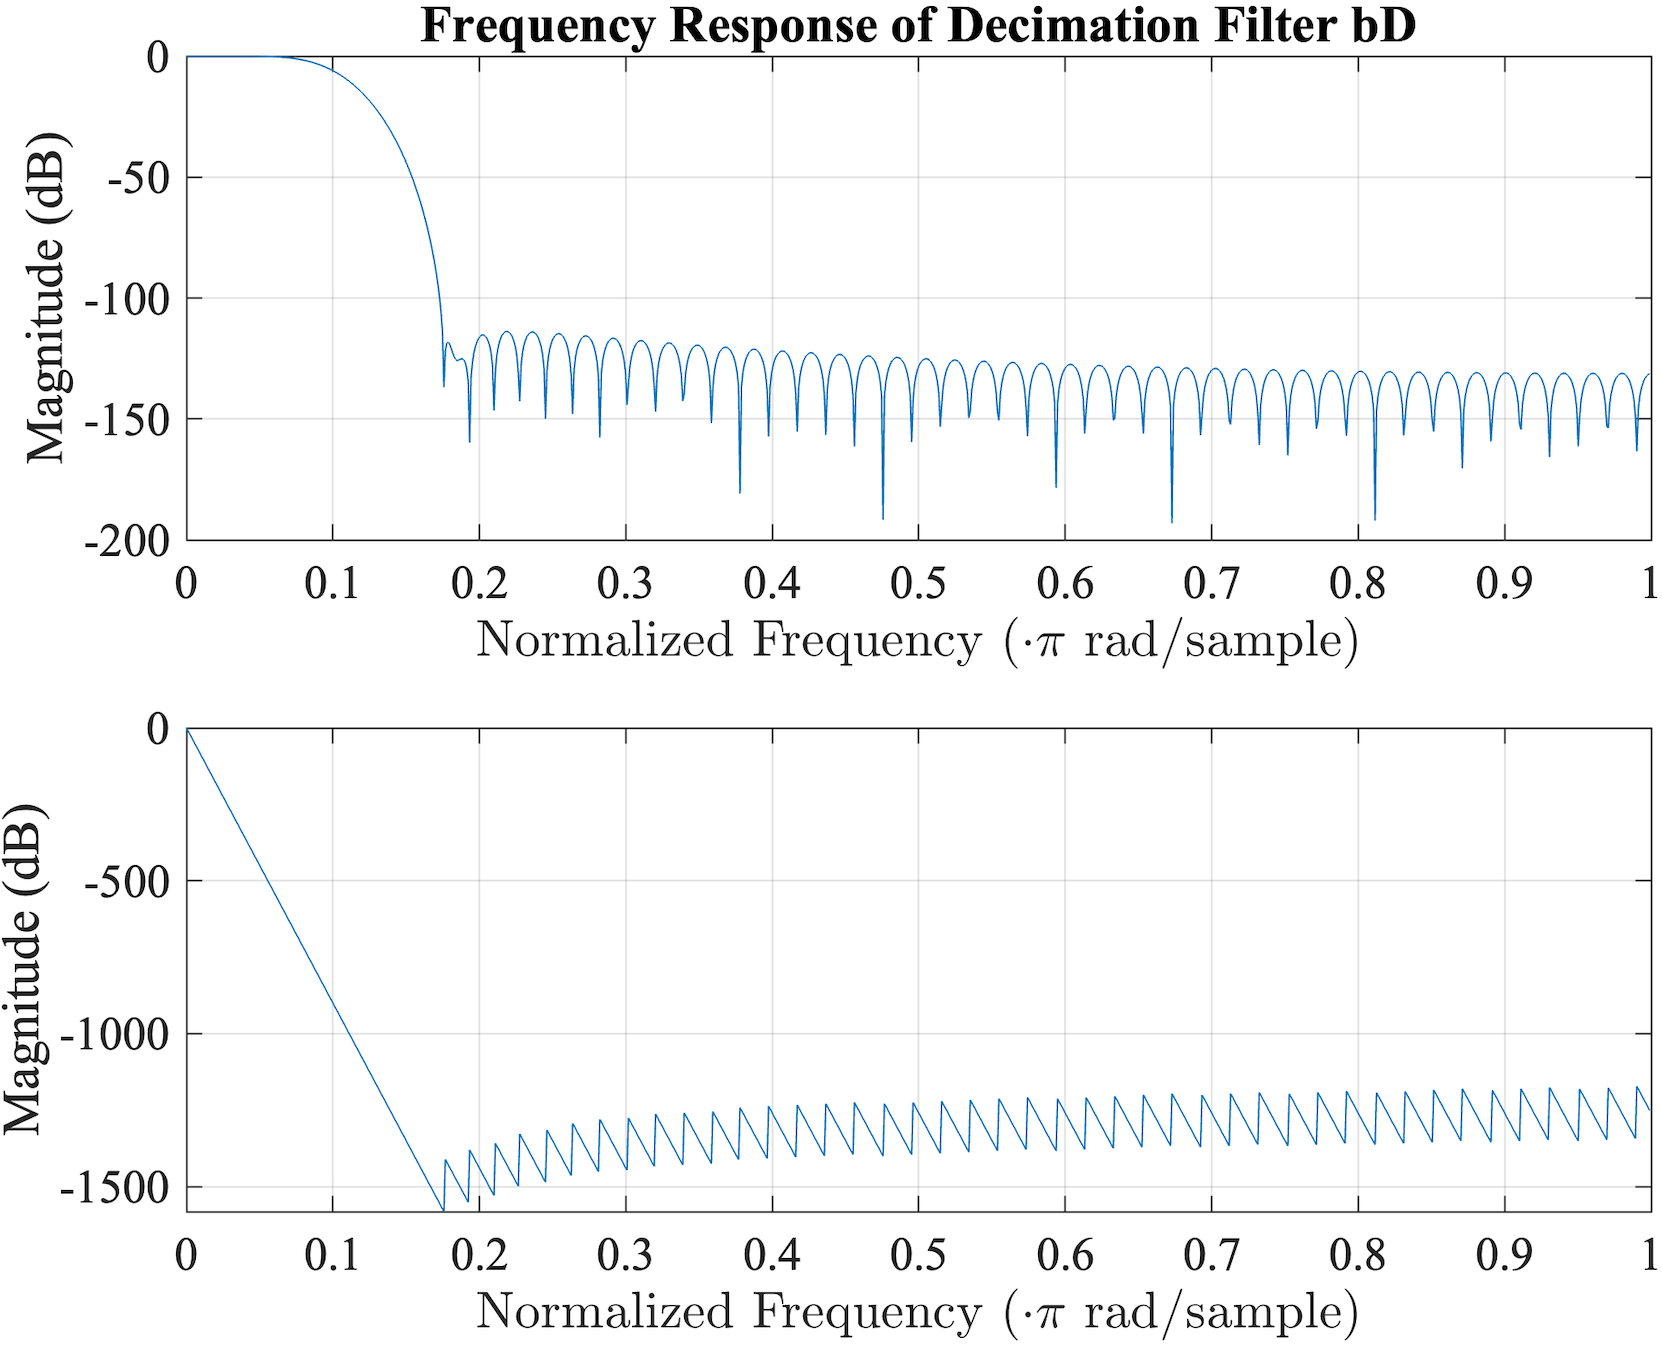
\includegraphics{img/Task_4_2.png}
  \captionof{figure}{Фильтр для N = 3 и N = 12}
\end{center}

\subsection*{2.5 Задание 5}
Для преобразования частоты дискретизации аудиосинала с нецелым шагом
необходимо разработать MATLAB-функцию расчёта параметра $L$ для интерполяции и
параметра $M$ для децимации сигнала.

\lstinputlisting[language=TeX]{code/functions/find_resample_step.m}

\subsection*{2.6 Задание 6}
Необходимо разработать MATLAB-функцию преобразования частоты дискретизации
с нецелым шагом в соответствии с алгоритмом.

\lstinputlisting[language=TeX]{code/functions/resample_audio.m}

\subsection*{2.7 Задание 7}
При помощи разработанной функции resample\_audio необходимо 
выполнить преобразование частоты дискретизации аудиосигнала в 
соответствии с вариантом. Аудифоайл «FA06\_01.wav».
Исходная частота дискретизации $f_s$ = 48000 Гц.
Требуемая частота дискретизации $f_s$ = 32000 Гц.

\lstinputlisting[language=TeX]{code/task7.m}

\subsection*{2.8 Задание 8}
Построить временное представление исходного сигнала и сигнала с изменённой
частотой дискретизации.

\lstinputlisting[language=TeX]{code/task8.m}

  Результат построения фильтра представлен 
на рисунке 3.
\begin{center}
  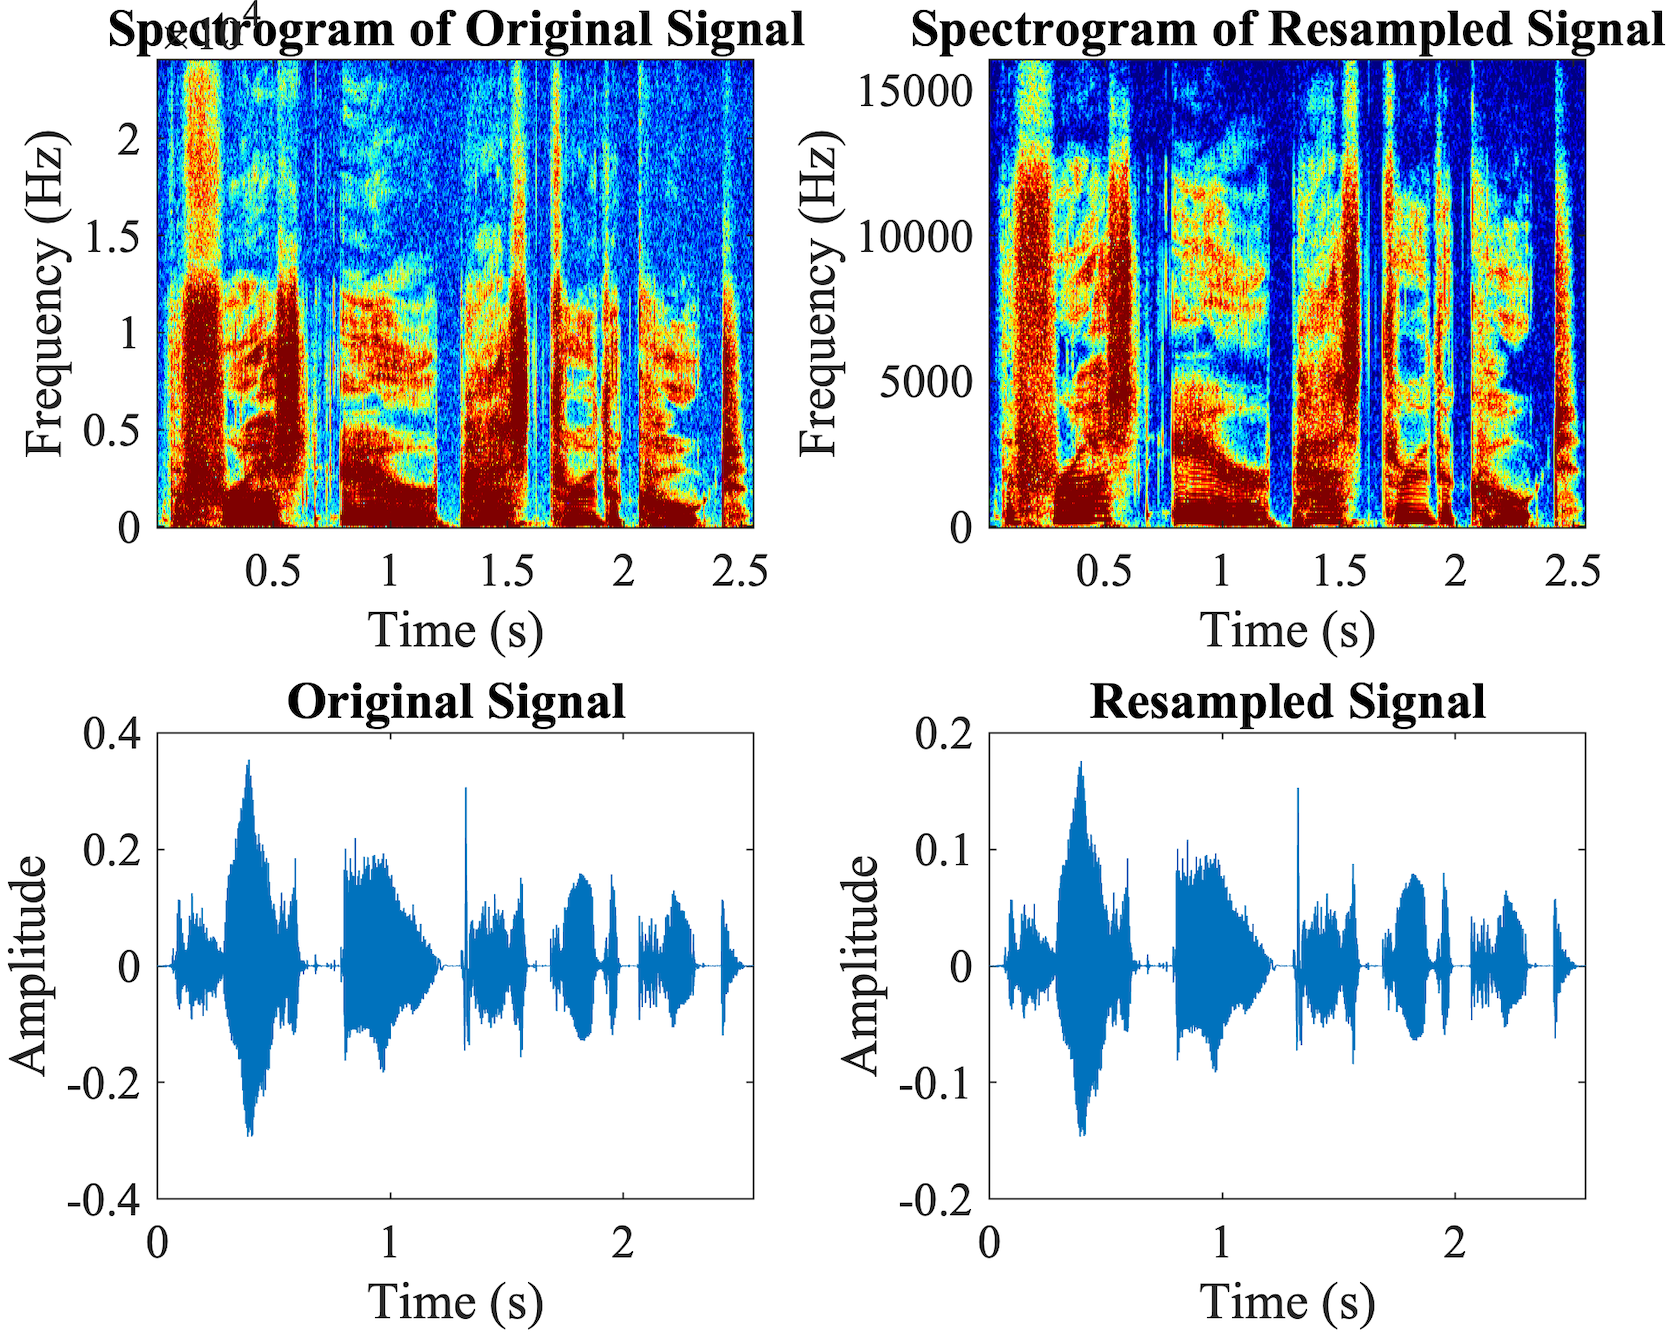
\includegraphics{img/Task_8.png}
  \captionof{figure}{Результат смены частоты дискретизации}
\end{center}

\section*{3 ВЫВОД}

  В результате выполнения лабораторной работы были получены 
практические навыки работы с аудио сигналами. Рассмотрен принцип работы АЦП.

\end{document}
